\documentclass{article}
\usepackage{graphicx}
\begin{document}
\begin{titlepage}
    \centering
    \vspace*{1cm}
    
    % Título
    \LARGE\textbf{UNIVERSIDAD TECNOLÓGICA DE TIJUANA}
    
    
\includegraphics[width=5cm]{LOGO.jpeg}
    \vspace{0.5cm}
    
   \LARGE\textbf{MATERIA: Diseño de App}

    \vspace{0.5cm}

     \LARGE\textbf{PROFESOR(A): Ray Brunett Parra Galaviz }
    \vspace{0.5cm}
    
    \LARGE\textbf{GRUPO: 4A BIS }

        % Subtítulo
    \LARGE\textbf{SRS}
    
   \vspace{0.5cm}

    % Autor y Afiliación
    \Large
    Autores: \\
    Alvarez Martinez Brayan Javier \\
    Barraza Andalón Kevin Giovanni\\
    Castillo Mendez Josue Leonel \\
    Farrera Martinez Ana Karen\\
    Samonte Mercado Jeremy\\
    
    
    \vspace{1cm}
    
    % Fecha
    \large
    Fecha de Entrega:  \today
    
    \vfill
    
    % Pie de página
    \begin{flushright}
        Versión 1.0
    \end{flushright}
\end{titlepage}

\section{Introducción}

En México, el sector de la construcción experimenta un constante crecimiento y una creciente demanda de maquinaria pesada, impulsada tanto por proyectos industriales como inmobiliarios. La renta de maquinaria se ha convertido en una solución recurrente para desarrollar nuevos proyectos de construcción, ya sean de pequeña escala o a largo plazo.\par. 

No obstante, el proceso de alquiler en el país a menudo se ve afectado por desafíos que van desde la falta de transparencia en la disponibilidad de maquinaria hasta tarifas y condiciones contractuales ambiguas. Esta situación puede dar lugar a malentendidos y disputas entre las partes involucradas.\par.

Este contexto ofrece la oportunidad de aplicar nuevas tecnologías para automatizar y simplificar el alquiler de maquinaria pesada mediante una plataforma web. La implementación de una plataforma en línea permitiría a las empresas y contratistas buscar, comparar y alquilar maquinaria de manera más eficiente, con un mayor grado de control y transparencia.\par.

Esta tesina se enfocará en explorar cómo la tecnología puede transformar el sector de alquiler de maquinaria pesada en México, abordando los desafíos existentes y proponiendo soluciones que beneficien a todos los actores involucrados en este importante mercado.\par

\section{Propósito}

Desarrollar una página web para que el cliente haga sus reservas desde casa con la información en la web más sencilla y fácil de usar.

\subsection{Objetivos Específicos}
\begin{enumerate}
    \item Optimizar el uso de maquinaria: Actuar para maximizar su eficiencia y productividad, asegurándonos de que la máquina esté siendo utilizada a su mayor capacidad y se le esté dando el uso adecuado.
    \item Programación eficiente: Desarrollar una plataforma web para asegurar que la máquina esté siendo utilizada el mayor tiempo posible y evitar que se encuentre inactiva por largos periodos.
    \item Mantenimiento del equipo: Implementar una solución de software que garantice que la maquinaria existente para renta esté bien y tenga una vida útil prolongada.
    \item Ampliación de oferta: Buscar oportunidades de atraer más proveedores con el fin de conseguir un catálogo más robusto y cubrir la mayor demanda posible.
    \item Analizar la situación actual: El documento pretende hacer un análisis exhaustivo de la situación actual del sector de alquiler de maquinaria pesada para la construcción. Esto implica identificar las fortalezas, debilidades, oportunidades y problemas que enfrentan las empresas.
\end{enumerate}

\subsection{Requerimientos Funcionales}
\begin{center}
\begin{tabular}{|p{3cm}|p{9cm}|}
\hline
\textbf{Requerimiento} & RF-C-001 \\
\hline
\textbf{Descripción} & Implementar un carrito de compra donde la cliente, una vez iniciada su sección de usuario, pueda agregar maquinaria para luego reservar. \\
\hline
\textbf{Nombre del requisito} & Carrito de compras \\
\hline
\textbf{Prioridad del requisito} & Alta/Esencial \\
\hline
\textbf{Persona asignada} & Castillo Mendez Josue Leonel \\
\hline
\end{tabular}
\end{center}

\begin{center}
\begin{tabular}{|p{3cm}|p{9cm}|}
\hline
\textbf{Requerimiento} & RF-C-002 \\
\hline
\textbf{Descripción} & Una vez el cliente agregó las máquinas que desea rentar, agregar información a un formulario para obtener datos como fecha de inicio y fin del alquiler, número de contacto, personal que recibirá la maquinaria y domicilio donde se entregará la maquinaria pesada una vez rentada. \\
\hline
\textbf{Nombre del requisito} & Formulario de reserva de maquinaria pesada \\
\hline
\textbf{Prioridad del requisito} & Alta/Esencial \\
\hline
\textbf{Persona asignada} & Farrera Martinez Ana Karen \\
\hline
\end{tabular}
\end{center}

\begin{center}
\begin{tabular}{|p{3cm}|p{9cm}|}
\hline
\textbf{Requerimiento} & RF-C-003 \\
\hline
\textbf{Descripción} & En la página principal, el cliente como usuario puede ver la maquinaria disponible para alquiler y su costo. \\
\hline
\textbf{Nombre del requisito} & Catálogo de maquinaria \\
\hline
\textbf{Prioridad del requisito} & Alta/Esencial \\
\hline
\textbf{Persona asignada} & Castillo Mendez Josue Leonel \\
\hline
\end{tabular}
\end{center}

\begin{center}
\begin{tabular}{|p{3cm}|p{9cm}|}
\hline
\textbf{Requerimiento} & RF-C-004 \\
\hline
\textbf{Descripción} & Implementar un menú donde el usuario podrá ver el saldo restante de la deuda del alquiler de la maquinaria rentada. \\
\hline
\textbf{Nombre del requisito} & Consulta de adeudo pendiente \\
\hline
\textbf{Prioridad del requisito} & Alta/Esencial \\
\hline
\textbf{Persona asignada} & Farrera Martinez Ana Karen \\
\hline
\end{tabular}
\end{center}

\begin{center}
\begin{tabular}{|p{3cm}|p{9cm}|}
\hline
\textbf{Requerimiento} & RF-C-005 \\
\hline
\textbf{Descripción} & El cliente podrá realizar pagos así como ver los pagos restantes. \\
\hline
\textbf{Nombre del requisito} & Registro y seguimiento de pagos pendientes \\
\hline
\textbf{Prioridad del requisito} & Alta/Esencial \\
\hline
\textbf{Persona asignada} & Castillo Mendez Josue Leonel \\
\hline
\end{tabular}
\end{center}

\begin{center}
\begin{tabular}{|p{3cm}|p{9cm}|}
\hline
\textbf{Requerimiento} & RF-C-006 \\
\hline
\textbf{Descripción} & Se mostrará un seguimiento de la reserva del alquiler de la maquinaria, así como el estado en la que se encuentra. \\
\hline
\textbf{Nombre del requisito} & Seguimiento de reservas en curso  \\
\hline
\textbf{Prioridad del requisito} & Alta/Esencial \\
\hline
\textbf{Persona asignada} & Farrera Martinez Ana Karen \\
\hline
\end{tabular}
\end{center}

\begin{center}
\begin{tabular}{|p{3cm}|p{9cm}|}
\hline
\textbf{Requerimiento} & RF-C-007 \\
\hline
\textbf{Descripción} & El usuario podrá ver las reservas hechas anteriormente y ver el registro de lo que se alquiló, así como su costo. \\
\hline
\textbf{Nombre del requisito} & Historial de reservas \\
\hline
\textbf{Prioridad del requisito} & Media \\
\hline
\textbf{Persona asignada} & Alvarez Martinez Brayan Javier \\
\hline
\end{tabular}
\end{center}

\begin{center}
\begin{tabular}{|p{3cm}|p{9cm}|}
\hline
\textbf{Requerimiento} & RF-C-008 \\
\hline
\textbf{Descripción} & Inicio de sesión, según el rol que tenga asignado el usuario, podrá ingresar a la plataforma de alquiler o ingresar al panel del admin. \\
\hline
\textbf{Nombre del requisito} & Inicio de sección para administradores, clientes y representantes de rentas \\
\hline
\textbf{Prioridad del requisito} & Alta/Esencial \\
\hline
\textbf{Persona asignada} & Barraza Andalón Kevin Giovanni \\
\hline
\end{tabular}
\end{center}

\begin{center}
\begin{tabular}{|p{3cm}|p{9cm}|}
\hline
\textbf{Requerimiento} & RF-C-009 \\
\hline
\textbf{Descripción} & Cualquier usuario contará con la opción de cerrar su sesión. \\
\hline
\textbf{Nombre del requisito} & Logout \\
\hline
\textbf{Prioridad del requisito} & Alta/Esencial \\
\hline
\textbf{Persona asignada} & Barraza Andalón Kevin Giovanni \\
\hline
\end{tabular}
\end{center}

\begin{center}
\begin{tabular}{|p{3cm}|p{9cm}|}
\hline
\textbf{Requerimiento} & RF-C-010 \\
\hline
\textbf{Descripción} & Solo el administrador podrá registrar nueva maquinaria. \\
\hline
\textbf{Nombre del requisito} & Alta de maquinaria por administradores \\
\hline
\textbf{Prioridad del requisito} & Alta/Esencial \\
\hline
\textbf{Persona asignada} & Barraza Andalon Kevin Giovanni \\
\hline
\end{tabular}
\end{center}

\begin{center}
\begin{tabular}{|p{3cm}|p{9cm}|}
\hline
\textbf{Requerimiento} & RF-C-011 \\
\hline
\textbf{Descripción} & Solo el administrador podrá dar de baja la maquinaria, tomando en cuenta que no se encuentre en renta o mantenimiento. \\
\hline
\textbf{Nombre del requisito} & Baja de maquinaria por administradores \\
\hline
\textbf{Prioridad del requisito} & Alta/Esencial \\
\hline
\textbf{Persona asignada} & Samonte Mercado Jeremy \\
\hline
\end{tabular}
\end{center}

\begin{center}
\begin{tabular}{|p{3cm}|p{9cm}|}
\hline
\textbf{Requerimiento} & RF-C-012 \\
\hline
\textbf{Descripción} & La implementación de dispositivos físicos, como el sistema de posicionamiento global (GPS), tendrá un enfoque hacia la seguridad mejorada en el seguimiento de maquinaria alquilada. \\
\hline
\textbf{Nombre del requisito} & GPS tracking \\
\hline
\textbf{Prioridad del requisito} & Alta/Esencial \\
\hline
\textbf{Persona asignada} & Samonte Mercado Jeremy \\
\hline
\end{tabular}
\end{center}

\begin{center}
\begin{tabular}{|p{3cm}|p{9cm}|}
\hline
\textbf{Requerimiento} & RF-C-013 \\
\hline
\textbf{Descripción} & Portear la página web de renta de maquinaria a móvil con el framework React Native. \\
\hline
\textbf{Nombre del requisito} & Página en móvil \\
\hline
\textbf{Prioridad del requisito} & Alta/Esencial \\
\hline
\textbf{Persona asignada} & Samonte Mercado Jeremy \\
\hline
\end{tabular}
\end{center}

\begin{center}
\begin{tabular}{|p{3cm}|p{9cm}|}
\hline
\textbf{Requerimiento} & RF-C-014 \\
\hline
\textbf{Descripción} & Implementación de APIs para facilitar servicios como API de Google para login y un API para localización GPS. \\
\hline
\textbf{Nombre del requisito} & APIs \\
\hline
\textbf{Prioridad del requisito} & Alta/Esencial \\
\hline
\textbf{Persona asignada} & Alvarez Martinez Brayan Javier \\
\hline
\end{tabular}
\end{center}

\subsection{Requerimientos NO funcionales}
\begin{center}
\begin{tabular}{|p{3cm}|p{9cm}|}
\hline
\textbf{Requerimiento} & RNF-001 \\
\hline
\textbf{Descripción} & El usuario en la página principal podrá realizar búsquedas avanzadas, tomando en cuenta marca, capacidad de carga y precio. \\
\hline
\textbf{Nombre del requisito} & Búsqueda y filtrado de máquinas. \\
\hline
\textbf{Prioridad del requisito} & Baja \\
\hline
\textbf{Persona asignada} & Farrera Martinez Ana Karen \\
\hline
\end{tabular}
\end{center}

\begin{figure}
\section{Diagramas}
    \centering
    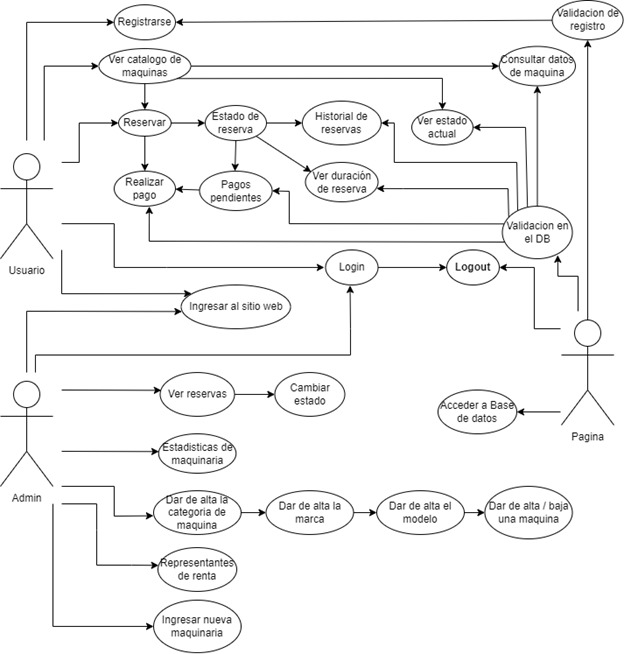
\includegraphics[width=1.1\linewidth]{Casos.jpg}
    \caption{Casos de uso}
    \label{fig:enter-label}
\end{figure}

\begin{figure}
    \centering
    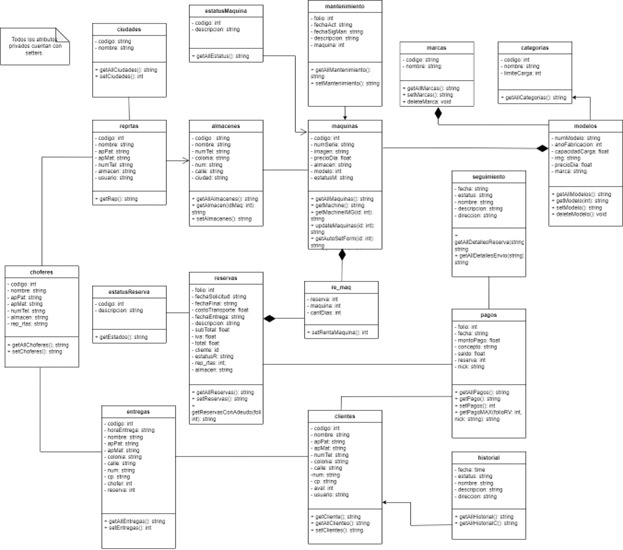
\includegraphics[width=1.1\linewidth]{clases.jpg}
    \caption{Diagrama de clases}
    \label{fig:enter-label}
\end{figure}
\begin{figure}
    \centering
    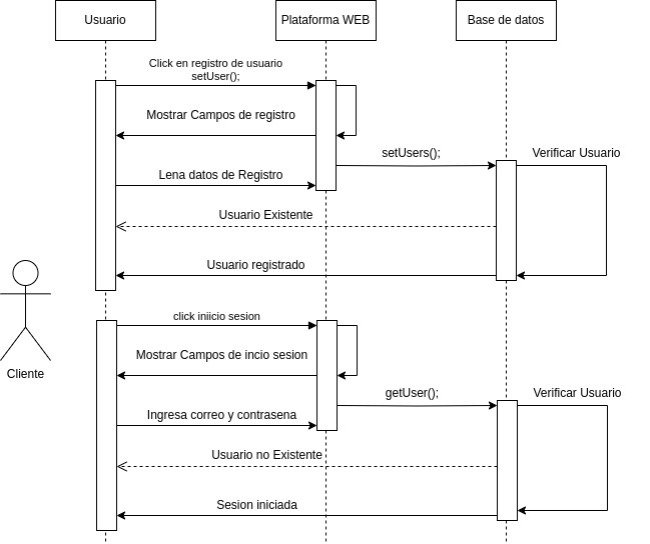
\includegraphics[width=1.1\linewidth]{sec1.jpg}
    \caption{Diagrama de secuencia 1}
    \label{fig:enter-label}
\end{figure}

\begin{figure}
    \centering
    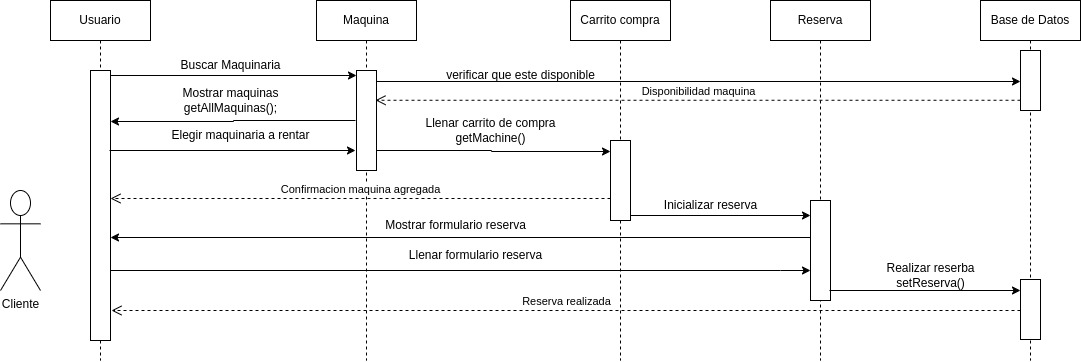
\includegraphics[width=1.1\linewidth]{sec2.jpg}
    \caption{Diagrama de secuencia 2}
    \label{fig:enter-label}
\end{figure}

\begin{figure}
    \centering
    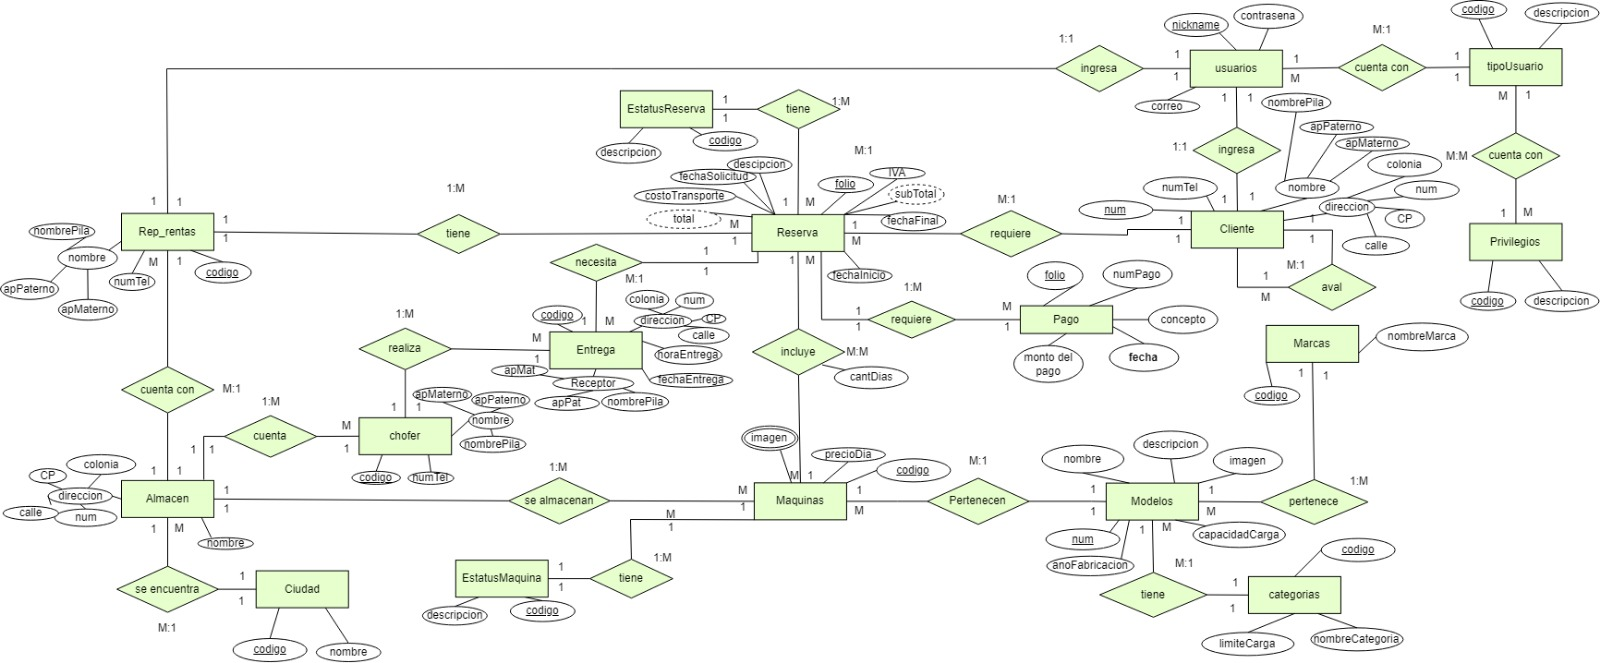
\includegraphics[width=1.2\linewidth]{der.jpg}
    \caption{Diagrama entidad relación}
    \label{fig:enter-label}
\end{figure}

\begin{figure}
    \centering
    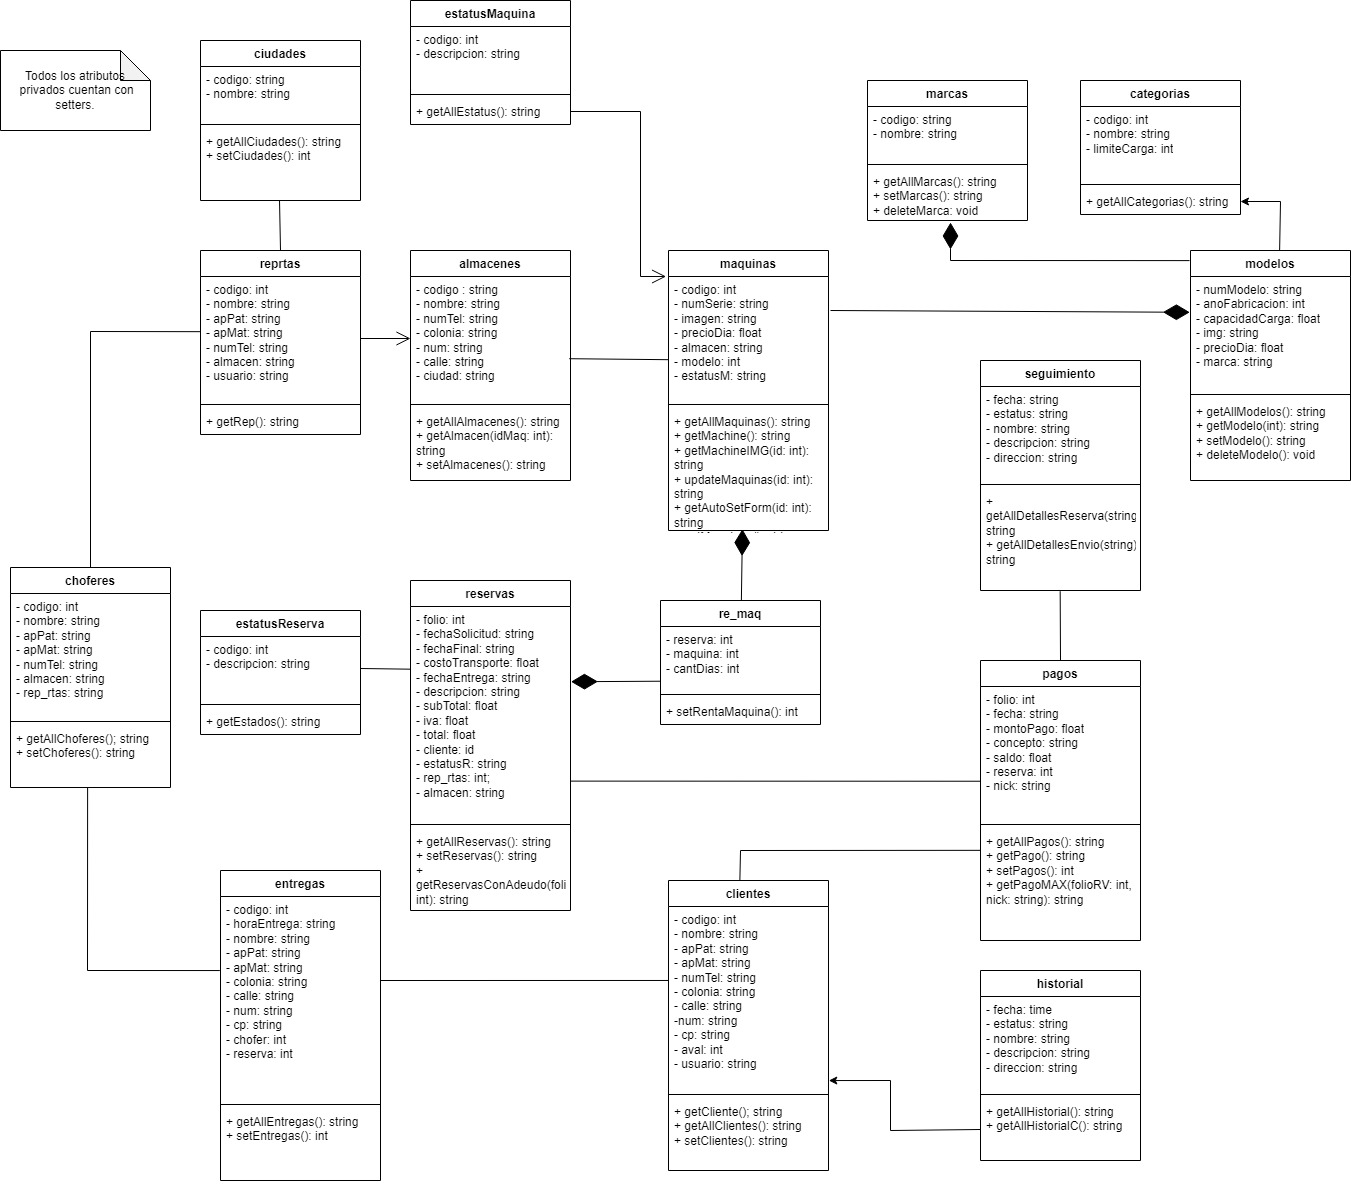
\includegraphics[width=1.1\linewidth]{mr.jpg}
    \caption{Modelo relacional}
    \label{fig:enter-label}
\end{figure}

\begin{figure}
\section{Maquetado}
    \centering
    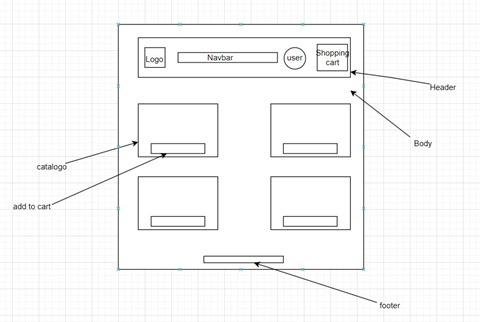
\includegraphics[width=1.1\linewidth]{pag.jpg}    \caption{Página principal}
    \label{fig:enter-label}
\end{figure}

\begin{figure}
    \centering
    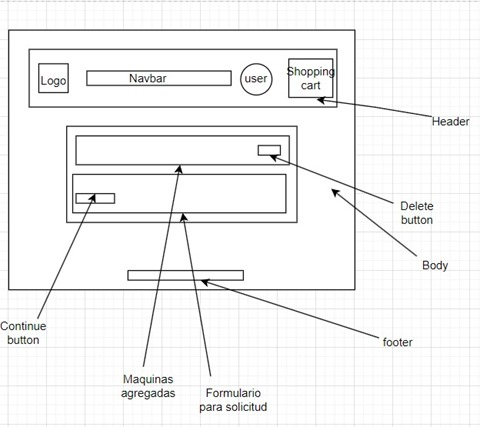
\includegraphics[width=1.1\linewidth]{2.jpg}
    \caption{Dentro de cart}
    \label{fig:enter-label}
\end{figure}
\begin{figure}
    \centering
    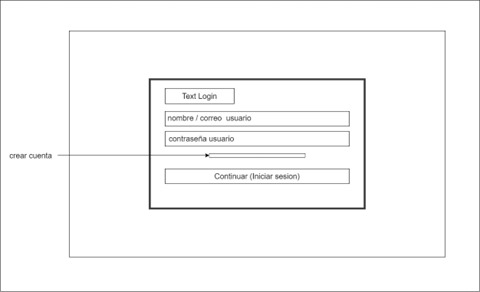
\includegraphics[width=1.1\linewidth]{3.jpg}
    \caption{Login de usuario}
    \label{fig:enter-label}
\end{figure}
\begin{figure}
    \centering
    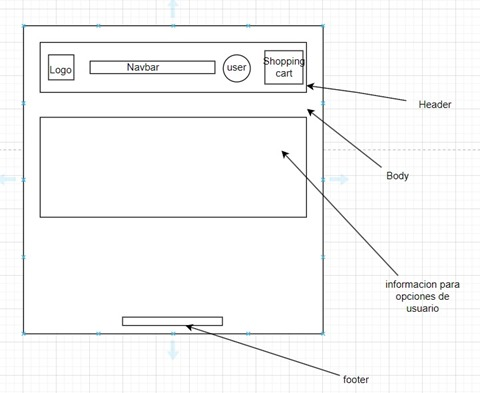
\includegraphics[width=1.1\linewidth]{3.5.jpg}
    \caption{Menú usuario}
    \label{fig:enter-label}
\end{figure}
\begin{figure}
    \centering
    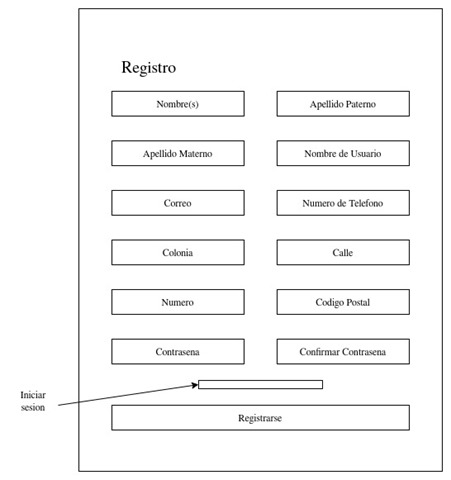
\includegraphics[width=1.1\linewidth]{4.jpg}
    \caption{Registro de usuario}
    \label{fig:enter-label}
\end{figure}
\begin{figure}
    \centering
    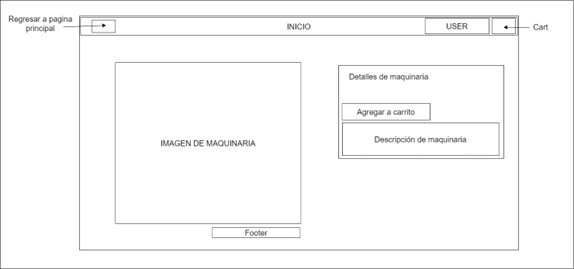
\includegraphics[width=1.1\linewidth]{5.jpg}
    \caption{Información de maquinaria interfaz (carrusel)}
    \label{fig:enter-label}
\end{figure}
\begin{figure}
    \centering
    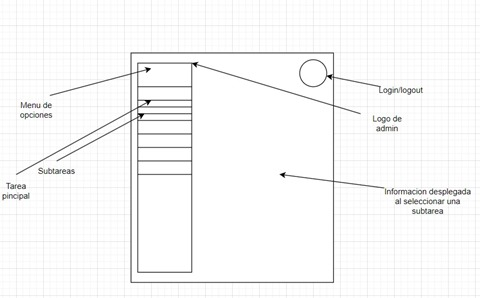
\includegraphics[width=1.1\linewidth]{6.jpg}
    \caption{Menú Admin}
    \label{fig:enter-label}
\end{figure}

\end{document}
